\documentclass[tikz,border=2pt]{standalone}
\usepackage{amsmath,amssymb}
\usepackage{tikz}
\usetikzlibrary{arrows.meta}

\begin{document}
% Diagonalizable: two independent eigen-directions (left). Defective: the shear has only one
% eigen-direction, so no eigenbasis exists (right).
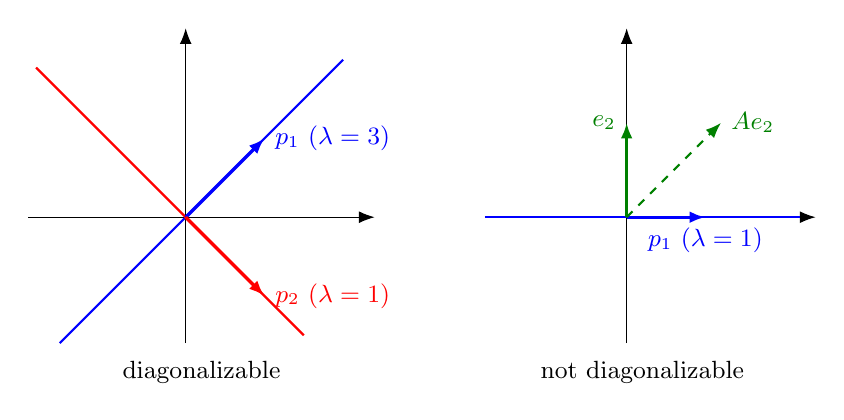
\begin{tikzpicture}[every node/.style={font=\small}, >={Latex[length=2mm]}]
	\begin{scope}
		\draw[->] (-2.0,0) -- (2.4,0);
		\draw[->] (0,-1.6) -- (0,2.4);
		\draw[blue, thick] (-1.6,-1.6) -- (2.0,2.0);
		\draw[red, thick] (-1.9,1.9) -- (1.5,-1.5);
		\draw[->, blue, very thick] (0,0) -- (1,1) node[right] {$p_1$ ($\lambda=3$)};
		\draw[->, red, very thick] (0,0) -- (1,-1) node[right] {$p_2$ ($\lambda=1$)};
		\node[anchor=north] at (0.2,-1.7) {diagonalizable};
	\end{scope}
	\begin{scope}[xshift=5.6cm]
		\draw[->] (-1.8,0) -- (2.4,0);
		\draw[->] (0,-1.6) -- (0,2.4);
		\draw[blue, thick] (-1.8,0) -- (2.2,0);
		\draw[->, blue, very thick] (0,0) -- (1,0) node[below] {$p_1$ ($\lambda=1$)};
		\draw[->, green!50!black, very thick] (0,0) -- (0,1.2) node[left] {$e_2$};
		\draw[->, green!50!black, thick, dashed] (0,0) -- (1.2,1.2) node[right] {$Ae_2$};
		\node[anchor=north] at (0.2,-1.7) {not diagonalizable};
	\end{scope}
\end{tikzpicture}
\end{document}
